\chapter{THERMAL SOLUTIONS}
% !TEX root = hazy1.tex

\section{Overview}

This Chapter describes options that affect the thermal solution and the
gas kinetic temperature.

The accuracy of the thermal solution is set by the error tolerance in
the heating---cooling balance.
This is set with the \cdCommand{set temperature tolerance} command.
Other commands can change some details of the thermal solution.

\section{cextra -14.231 [temp to the 1.5 power]}

This adds an extra cooling term due to some unspecified physical process.
The first number is the log of the cooling rate [erg cm$^{-3}$~s$^{-1}$].  The second
number is an optional exponent that specifies a temperature dependence.
The cooling will be given by
\begin{equation}
\Lambda  = 10^{c_1 }  \times \left( {\frac{{T_e }}{{10^4 \;{\mathrm{K}}}}}
\right)^{c_2 }
[\mathrm{erg\ cm}^{-3} \mathrm{s}^{-1}]% (57)
\end{equation}
where $c_1$ and $c_2$ are the two numbers entered with this command. If the second
optional argument $c_2$ is not specified then zero
(i.e., constant cooling) is assumed.

The function evaluating \cdCommand{cextra} sets the
variable \cdVariable{cextxx}.
The expression can be easily changed to other forms by changing
how this variable is set.

\section{Constant temperature, t=1e4 K [linear]}

A constant gas kinetic temperature calculation will be performed.
The number
is the electron temperature and is interpreted
as the log
of the value if it is $\le$ 10 or if the keyword \cdCommand{log} is present.
The optional keyword \cdCommand{linear} forces
interpretation as a linear quantity.
The temperature must be within the temperature limits
of the code, currently \TEMPLIMITLOW~$\leq T \leq$~\TEMPLIMITHIGH.

By default the temperature is specified in Kelvin.
The keywords \cdCommand{eV}
and \cdCommand{keV} are also accepted.

Collisional ionization of all atoms and ions is included so this option
can be used to produce clouds in coronal or collisional equilibrium.

\cdTerm{WARNING!}  It is also necessary to specify a
stopping criterion of some
kind when this command is used.
Most thermal-equilibrium calculations stop
when the electron temperature falls below some lowest value, set with the
\cdCommand{stop temperature} command and with the default
value \TEMPSTOPDEFAULT.
This cannot happen with a constant-temperature model.
For
instance, a constant temperature model of a planetary nebula will
continue
until the default limit to the number of zones (now 1400) is reached.
The
\emph{vast} majority of the cloud will consist of predominantly
neutral gas well outside the hydrogen Str\"omgren sphere.
This gas will have a small ambient
level of ionization and emission due to collisional ionization.
The
resulting emission-line spectrum might be surprising since the neutral gas
contributes significant emission.

Any of the stopping criteria described in the
Chapter \cdSectionTitle{Stopping Criteria} can be used.
A more physical constant
temperature model of a ionized cloud could be done by using the
\cdCommand{stop efrac} command to stop the calculation when the hydrogen
ionization front is reached.

\section{Constant grain temperature 20K [linear]}

Normally the temperature of each grain material and size is determined
by balancing heating and cooling.  This command sets the grain temperature
to the indicated quantity.

If the \cdCommand{linear} keyword appears then the number
is interpreted as the linear temperature.
Otherwise numbers $\le 10$ are interpreted as a log
of the temperature.

Other aspects of the grain physics are controlled with the
\cdCommand{grain} command.

\section{Coronal equilibrium, T=1e7 K [linear]}
\label{sec:CommandCoronalEquilibrium}

Coronal equilibrium, in which the gas is collisionally ionized, is
assumed.
The number is interpreted as the log of the
gas kinetic temperature if the
argument is $\le 10$ or the keyword \cdCommand{log} is present, and the linear temperature otherwise.
The optional keyword
\cdCommand{linear} will force the interpretation as a linear temperature.  This holds
the electron temperature at the specified value.

It is necessary\footnote{In versions 87 and before
the \cdCommand{coronal} command set the zone thickness
to 1 cm and stopped after computing one zone.}
to also specify some sort of stopping criteria.
The calculation will probably continue until the default
limit to the number
of zones is reached if a stopping criterion is not specified.
As an example, the following would compute the properties of $1 \pcc$ of a
low density gas at a million degrees Kelvin:
\begin{verbatim}
coronal, T=1e6K
hden 0      # H density 1 cm^-3
set dr 0    # set zone thickness of 1 cm
stop zone 1 # do only one zone
\end{verbatim}

If this is the only energy source specified then it is considered
an intensity command.
Emission-line intensities will be predicted,
as described on page \pageref{sec:IntensityLuminosityCases},
unless a radius is also specified.

Figure \ref{fig:coronal} shows the soft X-ray line and
continuum emission predicted
from the input stream in the test case \cdFilename{ism\_hot\_brems.in}.

\begin{figure}
\centering
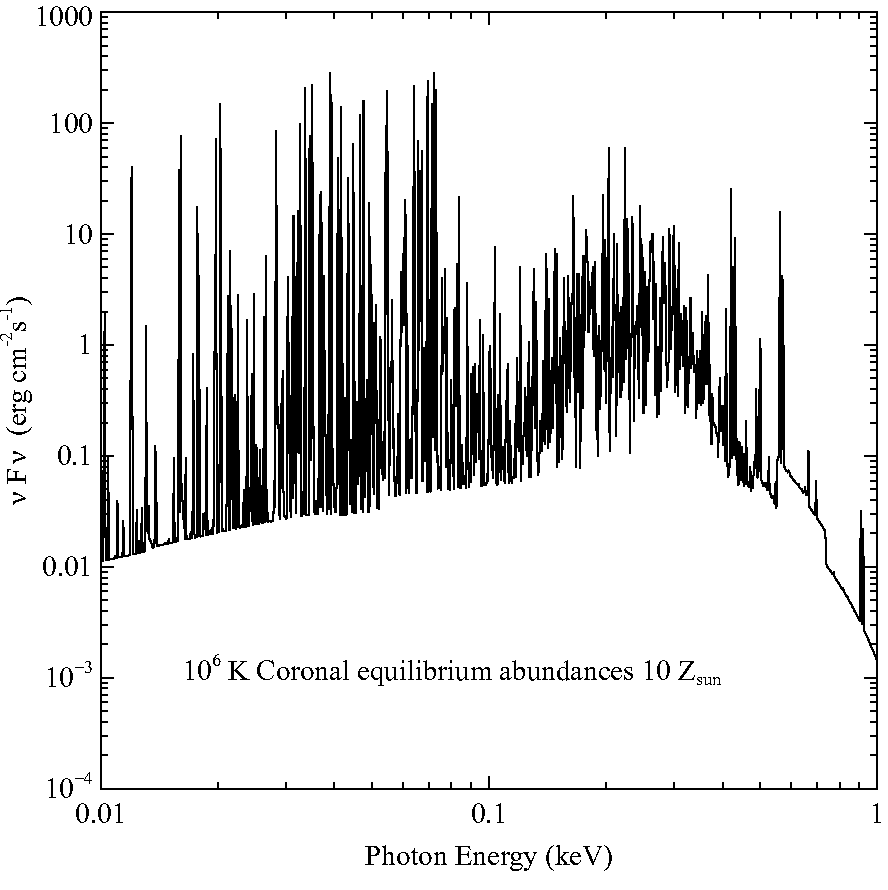
\includegraphics{coronal}
\caption[X-ray emission spectrum]
{\label{fig:coronal}This shows the soft X-ray emission from
the hot phase of a metal-rich ISM in coronal equilibrium.
The input script \cdFilename{ism\_hot\_brems.in} was used
to create the predicted spectrum. }
\end{figure}

The \cdCommand{time init} option provides a way to set initial conditions
for a time-dependent cloud.
This is described beginning on page 
\pageref{sec:TimeVariableRadiationFields}
where the \cdCommand{time} command is discussed.

\section{Cosmic rays [options.\dots]}

This adds cosmic rays and their heating and ionization.  
The command must be specified with at least the first five letters 
to avoid ambiguity with the \cdCommand{cosmology} command.

This physics
is described by \citet{FerlandMushotzky1984},
the subsection \cdSectionTitle{Cosmic Ray Interactions} in the section 
\cdSectionTitle{Other Physical Processes} in Part 3 of this
document, and section 11.3 of AGN3.
Cosmic rays mainly heat ionized gas
and both heat and create secondary ionizations in neutral gas.
All of this
is done self-consistently \citep{Dalgarno1999}.

The \cdCommand{set csupra} command provides a way to
specify an \hO\ secondary ionization rate.
This has many of the same effects
as introducing cosmic rays and uses the same code variables.
The rate
introduced by the \cdCommand{set csupra} command is not
self-consistent with the rest of the calculation but does
provide a way to test the code in certain simple limits.

Cosmic rays must be included if the calculation extends into molecular
regions.
The ion-molecule chemistry that occurs in the cold ISM requires
a source of ionization (\citealp{Dyson1997}).
In fact, most estimates
of the galactic cosmic ray background are based
on the abundances of chemical
ions such as H$_{3}^{+}$ (\citealp{McCall2003}; \citealp{Shaw2008}).
The chemistry
network will probably collapse if the gas becomes molecular
but cosmic rays
are not present.
The code will complain but try to compute the model if
a simulation without cosmic rays extends into cold gas.
If cosmic rays
are not included in the calculation and the neutral hydrogen ionization
rate falls below $10^{-17} \ps$
the code will print a comment stating that the
ionization rate fell below the galactic background rate.

\subsection{Cosmic rays background [1.2]}

This includes galactic background cosmic rays.
We adopt the \citet{Indriolo2007} mean \hO\ cosmic ray ionization rate 
of $2\times 10^{-16} \ps$.
The \htwo\ secondary ionization
rate is then $4.6\times 10^{-16} \ps$,\footnote{Before 2004 the code used a
background ionization rate of $7.4\times 10^{-18} \ps$
quoted by \citet[Table 10]{Tielens1985a}
and \citet{McKee1999}.
The rate of $2.5\times 10^{-17} \ps$ given by \citet{Williams1998} was used through
version C10.}.
(\citet{Glassgold.A74Model-calculations-for-diffuse-molecular} give the
relationship between \hO\ and \htwo\ ionization rates.)
\Cloudy\ determines the heating and
ionization rates of cosmic rays self consistently,
as appropriate for the
local molecular, atomic, and electron densities
(see AGN3 Section 11.3).

An optional scale factor specifies the cosmic ray ionization rate
relative to this background value.
The scale factor is assumed to be a
log unless the keyword \cdCommand{linear} also appears.

The background rate is an active research area.
\citet{McCall2003} find a background rate
$1.2 \times 10^{-15} \ps$ for a galactic
sight line.
\citet{Shaw2008} find a rate about five times larger from detailed
modeling of the sight line to Zeta Per.
\citet{Pellegrini2007} find a significantly enhanced ionization rate in M17.
\citet{Suchkov1993} find cosmic ray ionization rates that are
several dex larger than the galactic background in the starburst galaxy M82. 

\subsection{Cosmic ray rate -17.3}

If the keyword \cdCommand{rate} appears then the command specifies
the log of the
\hO\ ionization rate [s$^{-1}$] in predominantly neutral gas.
The default is
$2.5\times 10^{-17} \mathrm{s}^{-1}$ taken from \citet{Williams1998}.

\subsection{Cosmic rays density =1.2 [index, etc.]}

If the keyword \cdCommand{density} appears then the first number
is the log of the
cosmic ray density $n(cr)$~[cm$^{-3}$].
Expressions given in \citet{FerlandMushotzky1984} convert this into an ionization rate.

The second optional number is a power-law index $\alpha $ that
describes the
variation of the cosmic ray density with radius, i.e.,
\begin{equation}
n\left( {cr,\;r} \right) = n\left( {cr,\;r_o } \right)\left( {\frac{r}{{r_o
}}} \right)^\alpha
 [\mathrm{cm}^{-3}]  .
\end{equation}
The default value of the index is  $\alpha =0$,
corresponding to a constant cosmic-ray density.
The third optional number is the log of the temperature of
the fast electrons, if they are not relativistic.
If this third number
is specified then expressions from \citet{Balbus1982} will be used
to evaluate the electron heating rates.
The options can be omitted from right to left.

\subsection{Cosmic ray equipartition}

The cosmic rays are assumed to be in equipartition with the magnetic
field.
Then the cosmic-ray density is given by
\begin{equation}
n\left( {cr,\;B} \right) = n\left( {cr,\;B_{_0 } } \right)\left(
{\frac{{U\left( B \right)}}{{U\left( {B_0 } \right)}}} \right)
[\mathrm{cm}^{-3}]%   (59)
\end{equation}
where $U(B)$ and $U(B_0)$ are the energy densities of the local
magnetic field
relative to the galactic background magnetic field.
The \cdCommand{magnetic field}
command sets~$B$.  \citet{Webber1998} gives a cosmic-ray
energy density of 1.8~eV~cm$^{-3}$,
which corresponds to a magnetic field of
$8.5~\mu G$ if equipartition holds.
The background cosmic-ray ionization rate
is scaled by the ratio of the magnetic energy densities to find a local
cosmic ray ionization rate and energy density.

\subsection{The CR background and low-density gas}

The photoelectric heating and radiative cooling of low-density gas varies as the
square of the density while the CR heating varies linearly with density.
This means that CR effects become increasingly important, indeed dominant,
at low enough densities.
Figure \ref{fig:crDensityTemp} shows this.

The figure shows calculations in which both the galactic starlight and cosmic backgrounds 
are included.  
One set of calculations has the full cosmic ray background density while the second
has $10^{-5}$ of that value.  
The two nearly agree at high densities where CRs have little effect.
The effects of the CRs become increasingly dominant at lower densities, causing
the gas to reach temperatures of nearly $10^7$~K at the lowest hydrogen column density shown.

Something to think about before adding cosmic rays to simulations of low-density gas.

\begin{figure}
\centering
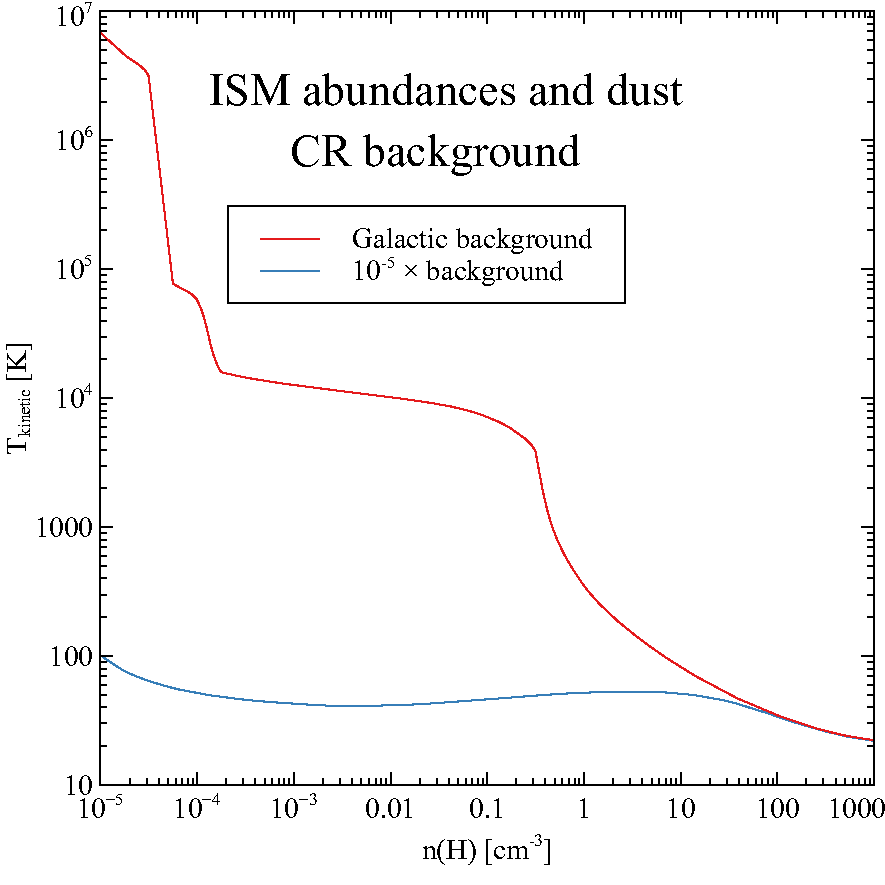
\includegraphics[scale=0.7]{crDensityTemp/crDensityTemp}
\caption[Effects of cosmic ray background on gas temperature]
{\label{fig:crDensityTemp}This shows  
the gas kinetic temperature as a function of hydrogen density for a parcel of ISM gas and dust
exposed to  ISM background starlight and cosmic rays.
The upper curve includes cosmic rays with the galactic background density while
the lower curve has a density $10^5$ times smaller.
The comsic rays strongly affect the conditions in the gas when the hydrogen density is below
$\sim 30 \pcc$.}
\end{figure}


\section{Failures 100 times [ map]}

A converge failure occurs when the heating-cooling balance,
the electron
density, or the pressure, is not within the tolerance set by the
\cdCommand{set convergence} commands.
Normally \Cloudy\ will
punt\footnote{FAQ:  Punt is a technical term from American football.
It is
something bad that happens when progress in advancing the ball is lacking.}
after an excessive number of convergence failures (presently 20)
occur.
This command increases the number of allowed failures to the value
entered as a parameter.

When \Cloudy\ stops because of excessive failures and the
\cdCommand{map} option is
specified\footnote{In versions 94 and before,
the default was to produce the map, and
the \cdCommand{no map} option turned this off.
With version 95 the option is not to
produce a map, and this must be requested with the
\cdCommand{map} option.}
as a keyword on the \cdCommand{failures} command it first
produces a map
of (heating-cooling) versus temperature to give an indication
of where the
equilibrium temperature should have been.
A section in Part 2 describes
thermal failures in more detail and describes this output.

Failures most often occur near a thermal front.
This occurs when the
solution jumps over peaks in the cooling function that occur near
$\sim2000 \K$ and $\sim 10^5 \K$.
A warning will be issued at the end of the calculation if
the global thermal balance is wrong.

It should not be necessary to use this command.
Please post the example
on the discussion board if you find a simulation where you need to
increase the number of convergence failures.

\section{Force temperature to 3400~K}

This forces the initial estimate of the temperature of the first zone
to the value entered.  The temperature is interpreted as a log if it is
$\le 10$ and the linear temperature otherwise.
The keywords \cdCommand{log} and \cdCommand{linear} will override this.

This command is useful if more than one initial temperature solution
is possible.
It forces the first guess of the temperature to the specified
value but \emph{does not} hold the temperature constant.
The temperature is
determined by energy balance thereafter.
(A constant kinetic temperature
is set with the \cdCommand{constant temperature} command.)

\Cloudy\ may have trouble finding a valid first temperature if the initial
solution is forced well away from the equilibrium value.
This is an
inevitable consequence of the complete linearization methods that are
intrinsic to the code's solvers.
If a large number of thermal failures
or warnings result from the use of this command then it is likely that the
code has been forced too far away from the solution.
A better guess of
the initial temperature would fix this problem.

\section{Hextra -14 [depth, density, time, SS]}

This includes extra heating due to some unspecified energy source.
The
first number $H_0$ is the log of the volume-heating rate
[erg~cm$^{-3}\mathrm{s}^{-1}$].
Optional keywords specify how this heating depends on density,
depth into the cloud, or time.
If these optional keywords do not occur then the heating
is constant.

\subsection{Hextra -14 depth 18, thickness 12}

The keyword \cdCommand{depth} makes the heating vary with depth
into the cloud.
The
second number is the log of the scale radius $r_{scale}$~[cm].
The extra heating
rate varies as\footnote{In versions through 94.00 the heating rate
varied as
$\exp[-r_{scale}/(r-r_o)]$ and went to infinity as the illuminated face.  The radial
dependence was changed to its current form in 94.01.}
\begin{equation}
H = H_0 [\exp ( - depth/r_{scale} ) + \exp (T - depth)/r_{scale} )]
 [\ergpccmps ].% (60)
\end{equation}
The third optional parameter $T$ is the total thickness of the slab.
If this
is given then the second exponential term will be added.
This will mimic
an external heat source that warms the cloud from both the illuminated and
shielded faces.
If the third parameter is not entered then the rightmost
term is not included.

\subsection{Hextra -13 density }

The \cdCommand{density} option makes the heating scale with the
hydrogen density.
The heating will be given~by
\begin{equation}
H = H_0 \left[ {n\left( \mathrm{H} \right)/n_0 } \right]
[\ergpccmps ].
\end{equation}
where $n$(H) is the local hydrogen density [cm$^{-3}$]
and $n_0$ is a scale density.
The scale density is unity by default and is changed by specifying the
optional second number, the log of the scale density.

\subsection{Hextra time}

If the \cdCommand{time} keyword appears then the variable
scale factors that appear
on the \cdCommand{time} command will multiply the heating
rate specified with the \cdCommand{hextra} command.
This makes it possible to follow
the effects of time-dependent heating sources.

\subsection{Hextra SS 0.2 1e8 3e17}

When the keyword \cdCommand{SS} appears, the standard $\alpha$-disk model
(\citet{Shakura1973}) will be used. The first parameter is $\alpha$, 
the dimensionless parameter of an $\alpha$-disk model. 
The second number is the mass of center black hole $M$ in solar mass units. 
The last one is the distance [cm] from the center of the disk $r$. 
In this model, heating rate is calculated as
\begin{equation}
H=\alpha P\sqrt{\frac{MG}{r^3}}[\ergpccmps]
\end{equation}
where $P$ is the local gas pressure [erg~cm$^{-3}$] 
and $G$ is gravitational constant. 
All three parameters must appear.
There are spaces to either side of
``\_\cdCommand{SS}\_''. 

\subsection{Notes on the hextra command}

The heating can only depend on depth or density
but the \cdCommand{time} option can
also be specified for each.

By default a calculation will stop when the kinetic temperature falls
below \TEMPSTOPDEFAULT.  It will be necessary to set other stopping criteria such
as the cloud thickness if the extra heating keeps the gas warmer than this
limit.

\section{High temperature approach}

This command tells the code to search for the first temperature by
approaching the thermal solution from the high temperature extreme of $10^6$~K.
Normally the approach is from low temperatures.
This can be useful
when more than one thermal solution is possible.
An example is shown in Figure 10 of \citet{FerlandFabian2009}.

\section{Magnetic field, log(B) = 5 [options]}

Magnetic fields are not included by default.
This specifies the strength
and geometry of the magnetic field.
A number, the log of the magnetic field
strength in Gauss, is the first number on the line.
The physical effects
of magnetic fields are discussed in Part 3 of this document.

Ordered and tangled fields can be specified.
The field is assumed to
be tangled by default.
If the keyword \cdCommand{ordered} appears then the angle between
the radiation field of the central object and the magnetic field
is also specified.
This angle is zero if the field is in the outward radial
direction.
The angle is given in degrees by default but the
\cdCommand{radian} keyword
will cause it to be radians instead.

In the case of a tangled field the code will look for a second number,
the index for the gamma-law relation between the magnetic field and the
gas density.
If a second number is not found then an index of $\gamma = 4/3$,
appropriate for a tangled field, will be assumed.
This index appears in the relationship
\begin{equation}
B_{{\mathrm{tangled}}}  = B_{{\mathrm{tangled}}}^0 \left( {\frac{\rho }{{\rho _0
}}} \right)^{\gamma /2}
 [\mathrm{Gauss}]
\end{equation}
where the term in parenthesis is the ratio of the current density to the
density at the illuminated face of the cloud.
For a spherical
constant-velocity flow, where ${\rho /\rho _0 }\propto(r/r_0 )^{-2} $, the
field will vary as  $B/B_0\propto( r/r_0 )^{-\gamma }$.
This is in contrast with a dipolar field,
in which the radial dependence
is $B/B_0 \propto( r /r_0 )^{-3}$.

Both ordered and tangled fields can be specified on separate commands.
If more than one ordered or tangled field is specified then the second
will take precedence over the first.

The major thermal effect of a field is to add cyclotron cooling.
This is only important at very high temperatures.

Magnetic pressure and enthalpy terms corresponding to the magnetic energy
density are included in the equation of state when a constant-pressure
geometry is assumed.
The magnetic pressure~is
\begin{equation}
P_B /k \approx \frac{{B^2 }}{{8\pi k}} \approx B_{100\,\mu G}^2
\;2.9 \times 10^6 [\pcc \K]
\end{equation}
where $B_{100\,\mu G}$ is
the magnetic field in units of $100\,\mu G$.
The plasma $\beta$ parameter, defined
as the local ratio of thermal to magnetic energy densities,
$\beta  = P_{gas} /P_{mag} $,
is printed in the summary of pressure contributions.
The field affects the dynamics of the gas when $\beta\le 1$.

Supersonic turbulence in rough energy equipartition with the magnetic
field is often observed in the cold ISM (\citealp{HeilesCrutcher2005}).
The
\cdCommand{turbulence} command has an
\cdCommand{equipartition} option
to set the turbulent velocity to a value in energy equipartition
with the magnetic field.
Although a general correlation is observed in the cold
neutral medium of the ISM, it is not thought to be a fundamental relationship (see the Heiles \& Crutcher paper).

\section{Map, zone 4 [range 2000, 5000]}

This computes the heating-cooling vs temperature relation (a ``thermal
map'') of the zone specified as the first number on the line.
This is one
way to check for the existence of more than one thermal solution.
If no
zone is specified, or if the zone is less than or equal to 0, then only
a thermal map is produced for the illuminated face of the cloud and the
calculation then stops.
The calculation of the heating and cooling is
self-consistent across this map.
A section in \cdTerm{Problems} in Part 2 of this
document explains how to interpret the map output.

The map produced by this command is not directly comparable to the more
typical plot that shows the equilibrium temperature as a function of
ionization parameter (\citealp{Krolik1981}).
That map can be
produced by successively calling \Cloudy\ with the same
radiation field
but different densities, say, with the \cdCommand{grid} command.
In that second case each deduced temperature is a valid
equilibrium temperature.
In the map produced by the \cdCommand{map} command only one
temperature, where heating and cooling are equal, is a valid equilibrium
temperature.
The map produced by this command is useful for checking for
more than one thermal solution,
to check that the heating and cooling curves
smoothly flow as the temperature changes,
or to investigate why the code
had convergence problems
(it was originally introduced for only this latter purpose).

The optional keyword \cdCommand{range} specifies the temperature
range of the map.
If this option is specified then the first number on the line must be the
zone for the map, zero if only a map of the illuminated face,
and the next two
numbers must be the lower and upper temperature limits to the map.
These temperatures
will be interpreted as logs if the first temperature is $\le 10$.  Normally
about 20 steps occur between the lowest and highest temperature in the map.
The number of steps can be reset with the \cdCommand{set nmaps} command.

The thermal map can be saved as a separate file with the
\cdCommand{save map} command.
This produces output that is suitable for
processing by other software.

The code stops when the map is complete since it is left in a disturbed
state.

\section{Neutrons -2 [efficiency =-2]}

This adds energy deposition and ionization by secondaries due to the
fast neutrons proposed by \citet{Sikora1989}.
The argument
is the luminosity in fast neutrons expressed as a fraction of the
\emph{total} photon luminosity of the incident continuum.
It is interpreted as a log
if $\le 0$ and a linear scale factor if positive.

The second optional argument is the heating---ionization efficiency
of the neutrons, unity by default.
Both quantities are interpreted as logs
if $\le 0$ and linear if positive.

\section{Print coolants, zone 135}

See the \cdCommand{print \dots} commands below.

\section{Print heating}

See the \cdCommand{print \dots} commands below.

\section{Set temperature [floor, convergence]}

See the \cdCommand{set temperature \dots} commands below.

\section{tlaw [DB96, SN99]}

This specifies a temperature law.
Two options currently are implemented.

The \cdCommand{DB96} option tells the code to use
the temperature---column density
law used by \citet{Draine1996}:
\begin{equation}
T = T_0 /\left[ {1 + N({\mathrm{H}})\,\sigma _{d{,}1000} } \right]
 [\K ]
\end{equation}
where $T_0$ is 500~K and $\sigma$ is $6\times 10^{-22} \pscm$.

The \cdCommand{SN99} option tells the code to use
the temperature - \htwo\ fraction
relationship assumed by \citet{Sternberg1999};
\begin{equation}
T = \frac{{500}}{{1 + 9\left[ {2n\left( {{\mathrm{H}}_2 } \right)/n\left(
{{\mathrm{H}}_{tot} } \right)} \right]^4 }}
 \; [\K].
\end{equation}

\subsection{Tlaw table [depth, radius]}

If the keyword \cdCommand{table} appears on the \cdCommand{tlaw}
command then the code will read
in a set of ordered pairs of radii and temperatures.
There must be two numbers per line
as in the example below.
The first number is the log of the radius or depth
[cm] and is followed by the log of the temperature [K].
If the
keyword \cdCommand{depth} also appears on the command line then
the first number is
interpreted as the log of the depth from the illuminated face
and the table
must begin with a depth smaller than 10$^{-30}$ cm,
the first point where the
depth is evaluated.
The first number is interpreted as the log of the radius
if \cdCommand{depth} does not appear.
The ordered pairs end with a line with the keyword
\cdCommand{end} in columns 1 through~3.

Linear interpolation in log-log space is done.
The following is an example.
\begin{verbatim}
tlaw table depth
continue -35 4
continue 12 4
continue 13 5
continue 14 6
continue 15 7
end of tlaw
\end{verbatim}

Be sure that the first and last radii or depths extend beyond the computed
geometry---this law is only be used for interpolation and the code will
stop if extrapolation is necessary.
Note that the first depth must be
smaller than $10^{-30}$~cm,
and also that there must not be a space in the first
column of any lines with numbers---the code will think that an end of file
has been reached.
Alphabetic characters can be placed anywhere on the line
and will be ignored---I placed the word
\cdCommand{continue} in the first four columns
for this reason (it is actually totally ignored).

